\documentclass[a4paper,10pt]{article}

% Encoding.
\usepackage{geometry}
\usepackage[T2A]{fontenc}
\usepackage[utf8]{inputenc}
\usepackage[english,russian]{babel}

\usepackage{hyperref}

\hypersetup{
    colorlinks,
    linkcolor=black,
    urlcolor=blue
}

% Code insertion.
\usepackage[outputdir=build]{minted}

% Math functions.
\usepackage{amsmath}

% Image insertion.
\usepackage{svg}

% No line breaks.
\usepackage[none]{hyphenat}

\title{Задание 3: план управления проектом ``e-гриб''}
\author{
    \begin{tabular}[t]{c@{\extracolsep{8em}}c} 
        Афанасов Артём     & Смирнов Александр \\
        &\\ 
        Струтовский Максим & Федор Жилкин
    \end{tabular}
}

\date{\today}

\begin{document}

\maketitle

\tableofcontents

\newpage

\section{О документе}

\subsection{Цели документа}

    \begin{itemize}
        \item Составить план развития проекта по продаже ЧГ\footnote{Чайный гриб};
    \end{itemize}

\subsection{Термины и определения}

    \begin{itemize}
        \item ЧГ: чайный гриб;
    \end{itemize}

\subsection{Другие документы}

    \begin{itemize}
        \item Описание проекта: \href{https://github.com/SmirnovAlexander/ProjectManagement/blob/master/ProductInvention/product_invention.pdf}{ссылка};
        \item Устав проекта: \href{https://github.com/SmirnovAlexander/ProjectManagement/blob/master/ProductRegulations/product_regulation.pdf}{ссылка};
    \end{itemize}


\section{Определение проекта}

\subsection{Идентификация проекта}

    \begin{itemize}
        \item Название: \textit{e}-гриб;
        \item Заказчик и спонсор проекта: ОАО ``Eco Slavic Fit''
        \item Исполнитель: ООО ``Камбуча-Рус'';
    \end{itemize}

\subsection{Постановка задачи}


Явные цели:

    \begin{itemize}
        \item Приложения под платформы:
            \begin{itemize}
                \item iOS;
                \item Android;
                \item Web;
                \item 3500 заказов ЧГ;
            \end{itemize}
        \item Произодство ЧГ:
            \begin{itemize}
                \item Ферма по производству ЧГ;
                \item 4000 ЧГ в день;
            \end{itemize}
        \item Организация доставки ЧГ до клиента:
            \begin{itemize}
                \item 3 склада в разных концах Санкт-Петербурга;
                \item Аутсорс доставки из складов;
            \end{itemize}
        \item Чистая прибыль 10 млн. руб. в месяц;
    \end{itemize}

Неявные цели:

    \begin{itemize}
        \item Разобраться в предметной области;
        \item Получение первичного опыта в управлении проектами.
    \end{itemize}




\subsubsection{Рамки проекта}

Делаем сами:

    \begin{itemize}
        \item Ферма по выращиванию ЧГ:
            \begin{itemize}
                \item Сформировать команду специалистов по ЧГ;
                \item Арендовать помещение для выращивания ЧГ;
                \item Купить оборудование для выращивания ЧГ;
                \item Наладить процессы по выращиванию ЧГ;
            \end{itemize}
        \item Нанять персонал:
            \begin{itemize}
                \item 5 программистов;
                \item 3 специалиста по ЧГ;
                \item 10 сотрудников фермы;
                \item 9 сотрудников складов;
                \item 3 маркетолога;
                \item 3 сотрудника службы поддержки;
            \end{itemize}
        \item Разрабока:
            \begin{itemize}
                \item Сформировать команду программистов;
                \item Арендовать офис;
                \item Разработать план по разработке;
                \item Наладить процессы по разработке;
            \end{itemize}
        \item Маркетинг:
            \begin{itemize}
                \item Сформировать команду;
                \item Составить план по продвижению продукта;
                \item Сформировать корпоративный бренд;
            \end{itemize}
        \item Доставка:
            \begin{itemize}
                \item Арендовать склады;
            \end{itemize}
        \item Поддержка:
            \begin{itemize}
                \item Продумать use-case ЧГ;
                \item Сформировать команду поддержки:
                    \begin{itemize}
                        \item В интернете;
                        \item По телефону.
                    \end{itemize}
                \item Помощь в случае заболевания.
            \end{itemize}
    \end{itemize}

Аутсорс:

    \begin{itemize}
        \item Нанять строителей для обустройства фермы ЧГ;
        \item Договориться с аутсорс доставкой;
    \end{itemize}

\subsubsection{WBS}

    \begin{itemize}
        \item WBS изображена на Рис. 1;
    \end{itemize}

    \begin{figure}[h]
        \centering
        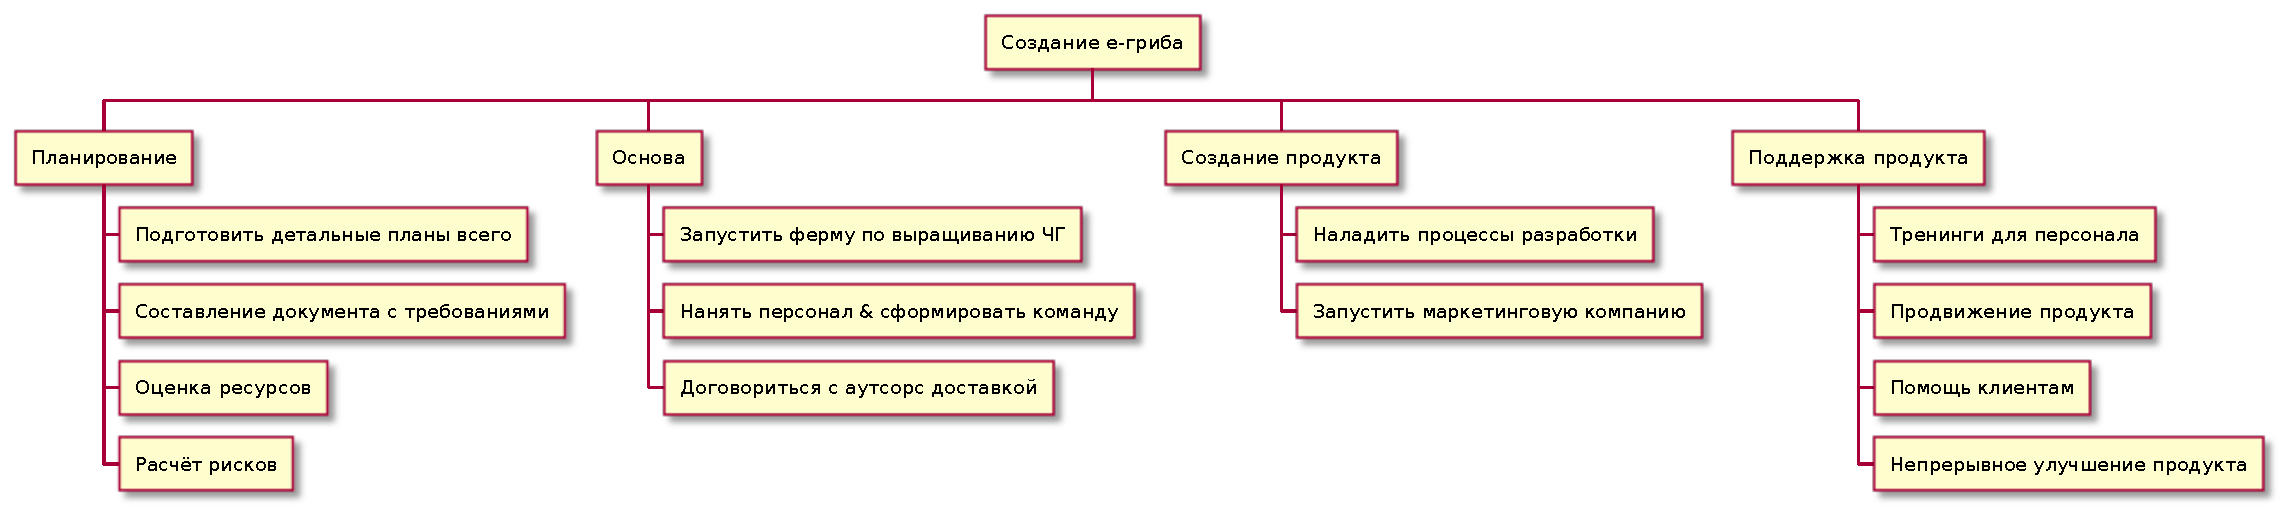
\includegraphics[width=1\textwidth]{./pics/wbs.pdf}
        \caption{wbs}
    \end{figure}

\subsubsection{Сроки проекта}

    \begin{itemize}
        \item 12 месяцев;
    \end{itemize}

\subsubsection{Основные фазы}



    \begin{itemize}
        \item Планирование:
            \begin{itemize}
                \item Подготовить детальные планы всего;
                \item Составление документа с требованиями;
                \item Оценка ресурсов;
                \item Расчёт рисков;
            \end{itemize}
        \item Основа:
            \begin{itemize}
                \item Запустить ферму по выращиванию ЧГ;
                \item Нанять персонал \& сформировать команду;
                \item Договориться с аутсорс доставкой;
            \end{itemize}
        \item Создание продукта:
            \begin{itemize}
                \item Наладить процессы разработки;
                \item Запустить маркетинговую компанию;
            \end{itemize}
        \item Поддержка продукта:
            \begin{itemize}
                \item Тренинги для персонала;
                \item Продвижение продукта;
                \item Помощь клиентам;
                \item Непрерывное улучшение продукта;
            \end{itemize}
    \end{itemize}




\subsubsection{Ресурсы}
    \begin{itemize}
        \item Оборудование:
            \begin{itemize}
                \item Оборудование для фермы;
                \item Складское оборудование;
                \item Офисное оборудование;
                \item Датчики \& лимонадники;
            \end{itemize}

        \item Аренда помещений:
            \begin{itemize}
                \item Ферма;
                \item 3 склада;
                \item Офис;
            \end{itemize}

        \item ПО:
            \begin{itemize}
                \item Microsoft Windows;
                \item Microsoft Office;
                \item Gitlab EE;
                \item Figma;
            \end{itemize}

        \item Финансовые ресурсы:
            \begin{itemize}
                \item Аутсорс доставки;
                \item Выплата ЗП.
            \end{itemize}

    \end{itemize}


\subsubsection{Ограничения}

    \begin{itemize}
        \item Финансы:
            \begin{itemize}
                \item 50 млн. руб.
            \end{itemize}
        \item Временные ограничения:
            \begin{itemize}
                \item 12 месяцев;
                \item Тренд на ЧГ;
                \item Конкуренция;
            \end{itemize}
        \item Ограничения по доставке:
            \begin{itemize}
                \item Санкт-Петербург.
            \end{itemize}
    \end{itemize}

\subsection{Критерии достижения цели}

    \begin{itemize}
        \item Приложения под платформы:
            \begin{itemize}
                \item iOS;
                \item Android;
                \item Web;
                \item 3500 заказов ЧГ в день;
            \end{itemize}
        \item Произодство ЧГ:
            \begin{itemize}
                \item Ферма по производству ЧГ;
                \item 4000 ЧГ в день;
            \end{itemize}
        \item Организация доставки ЧГ до клиента:
            \begin{itemize}
                \item 3 склада в разных концах Санкт-Петербурга;
                \item Аутсорс доставки из складов;
            \end{itemize}
        \item Чистая прибыль 10 млн. руб. в месяц.
    \end{itemize}


\subsection{Процедуры приёмки}

    \begin{itemize}
        \item Принимать работу будет комитет из заказчиков;
        \item Будет 2 митинга:
            \begin{itemize}
                \item После срока в 12 месяцев:
                    \begin{itemize}
                        \item Для понимания того, что было сделано;
                        \item Оценка готовности выхода на рынок;
                        \item Оценка пригодности использования;
                        \item По результатам оценок будет проходить сдача работ;
                    \end{itemize}
                \item После срока в 24 месяца:
                    \begin{itemize}
                        \item Чтобы оценить, как идут дела;
                        \item Анализ бизнес-отчётов;
                        \item Формирование дальнейшего плана продвижения;
                    \end{itemize}
            \end{itemize}
    \end{itemize}


\section{Организационная структура проекта}

\subsection{Заинтересованные лица и их ответственности}

    \begin{itemize}
        \item Заказчик и спонсор проекта: ОАО ``Eco Slavic Fit''
            \begin{itemize}
                \item Принятие стратегических решений;
                \item Предоставление ресурсов;
            \end{itemize}
        \item Исполнитель: ООО ``Камбуча-Рус'';
            \begin{itemize}
                \item Выработка и утверждение технических решений;
            \end{itemize}
        \item Директор: Смирнов М.Я.
            \begin{itemize}
                \item Администрирование
                \item Операционная деятельность
            \end{itemize}
        \item Пользователь
    \end{itemize}

\subsection{Команда проекта}

    \begin{itemize}
        \item 4 управленца:
            \begin{itemize}
                \item Куратор проекта (Смирнов А. Л.);
                \item Координатор проекта (Жилкин Ф. И.);
                \item Руководитель проекта (Струтовский М. Я.);
                \item Исполнительный директор проекта (Афанасов А. Ю.);
            \end{itemize}
        \item 5 программистов;
        \item 3 специалиста по ЧГ;
        \item 10 сотрудников фермы;
        \item 9 сотрудников складов;
        \item 3 маркетолога;
        \item 3 сотрудника службы поддержки;
    \end{itemize}

\subsection{Ресурсы проекта}


    \begin{itemize}
        \item Оборудование:
            \begin{itemize}
                \item Оборудование для фермы;
                \item Складское оборудование;
                \item Офисное оборудование;
                \item Датчики \& лимонадники;
            \end{itemize}

        \item Аренда помещений:
            \begin{itemize}
                \item Ферма;
                \item 3 склада;
                \item Офис;
            \end{itemize}

        \item ПО:
            \begin{itemize}
                \item Microsoft Windows;
                \item Microsoft Office;
                \item Gitlab EE;
                \item Figma;
            \end{itemize}

        \item Финансовые ресурсы:
            \begin{itemize}
                \item Аутсорс доставки;
                \item Выплата ЗП.
            \end{itemize}

    \end{itemize}


\section{Основные процедуры управления проектом}

\subsection{Типы отчётов}

    \begin{itemize}
        \item Ретроспетивы;
        \item Demo каждую неделю;
        \item Daily митинги;
        \item Финансовые отчёты;
        \item Отчёты с фермы;
        \item Отчёты от техподдержки;
    \end{itemize}


\subsection{Процедуры управления изменениями}

    \begin{itemize}
        \item Непрерывное взаимодействие с заказчиком
        \item Формирование требований для исполнителей
    \end{itemize}

\subsection{Процедуры анализа хода проекта}

    \begin{itemize}
        \item Спринты по 2 недели
        \item Финансовые отчёты каждый месяц
    \end{itemize}

\subsection{Методы планирования}

    \begin{itemize}
        \item Методология Kanban
        \item Ежедневные standup встречи по утрам
    \end{itemize}

\section{План управления коммуникациями}

\subsection{Участники коммуникации}

    \begin{itemize}
    \item Люди:
        \begin{itemize}
            \item Управленцы;
            \item Старший маркетолог;
            \item Старший сотрудник фермы;
            \item Старший программист;
            \item Старший специалист по ЧГ;
        \end{itemize}
    \item Организации:
        \begin{itemize}
            \item ОАО ``Eco Slavic Fit'';
            \item ООО ``Камбуча-Рус'';
        \end{itemize}
    \end{itemize}

\subsection{Способы коммуникации}

    \begin{itemize}
        \item Телефон;
        \item Почта;
        \item Zoom;
        \item Личные встречи;
    \end{itemize}

\subsection{График коммуникации}

    \begin{itemize}
        \item Ежедневные звонки и письма;
        \item Каждую пятницу Zoom-конференции;
        \item Личные встречи в конце каждого этапа работы над проектом;
    \end{itemize}

\subsection{Тех. средства коммуникации}

    \begin{itemize}
        \item Веб-камера;
        \item Микрофон;
    \end{itemize}

\section{План разработки}

\subsection{Фазы проекта}

    \begin{itemize}
        \item Старт:
            \begin{itemize}
                \item Сформированы команды;
                \item Арендованы складские помещения;
            \end{itemize}

        \item Подготовка к запуску производства:
            \begin{itemize}
                \item Подготовлено оборудование для выращивания ЧГ;
                \item Закуплены расходные материалы (удобрения, субстракт, споры);
                \item Разработано бета-ПО;
            \end{itemize}


        \item Запуск производства:
            \begin{itemize}
            \item Налажено выращивание ЧГ;
            \item Налажена доставка до логистических центров;
            \item Финальная версия ПО;
            \item Налажена связь со службой поддержки;
            \item Маркетологи начали рекламную кампанию;
            \end{itemize}

        \item Начало продаж:
            \begin{itemize}
                \item Налажена доставка до потребителя.
            \end{itemize}

    \end{itemize}


\subsection{Диаграмма Ганта}

    \begin{itemize}
        \item Диаграмма Ганта изображена на Рис. 2 (можно приближать);
    \end{itemize}


    \begin{figure}[h]
        \centering
        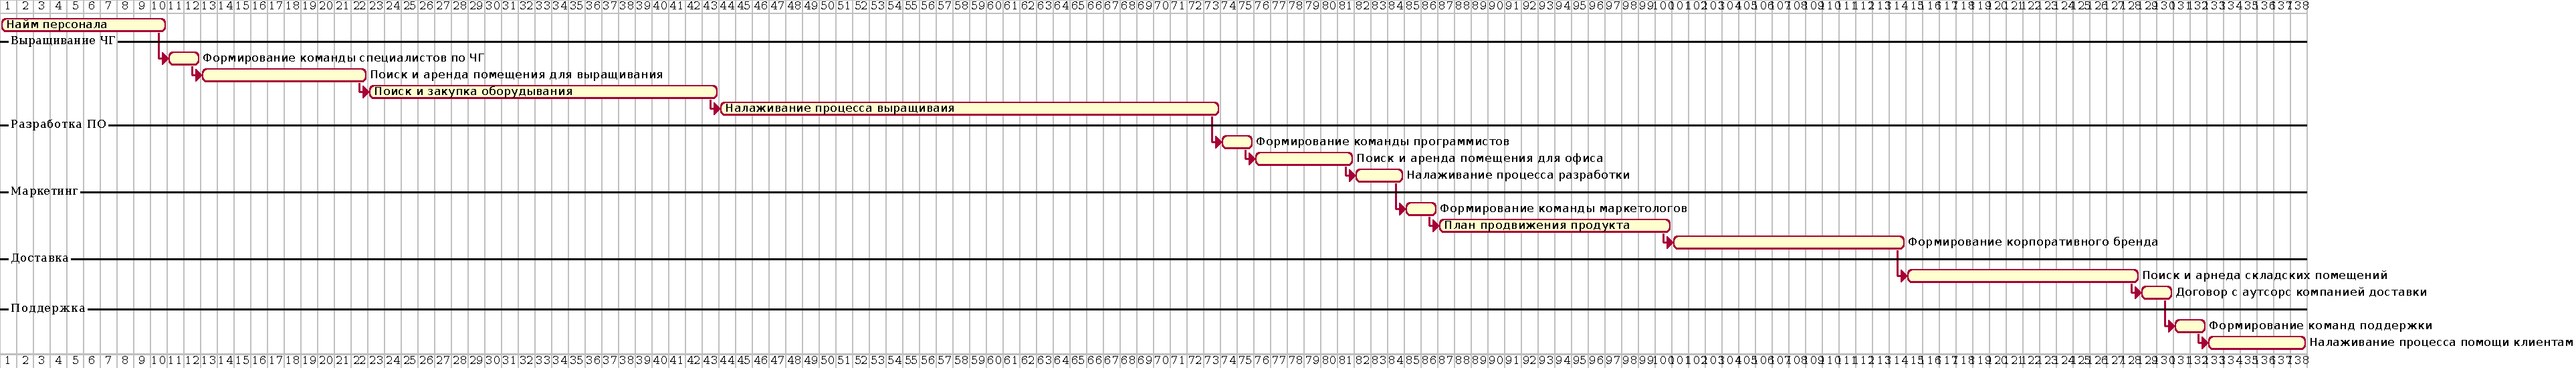
\includegraphics[width=1\textwidth]{./pics/gantt.pdf}
        \caption{gantt}
    \end{figure}



\section{Тестирование в проекте}

    \subsection{Тестирование системы}

        \begin{itemize}
            \item Функциональное:
                \begin{itemize}
                \item Проверка работоспособности ПО;
                \item Проверка корректности работы датчиков;
                \end{itemize}
            \item Регрессионное:
                \begin{itemize}
                    \item Тестирование работоспособности системы при расширении зоны продажи;
                \end{itemize}

            \item Приемочное:
                \begin{itemize}
                    \item Удовлетворение требованиям заказчика для принятия работы;
                \end{itemize}

            \item Нагрузочное:
                \begin{itemize}
                    \item Тестирование ПО при большой нагрузке пользователей;
                \end{itemize}

            \item Ответственный за тестирование системы:
                \begin{itemize}
                    \item Струтовский М.Я.;
                \end{itemize}
            \item Ошибки:
                \begin{itemize}
                    \item Ошибки отслеживаются ПО с помощью Jira;
                    \item Ошибки в производстве ЧГ заносятся в отчеты;
                \end{itemize}

        \end{itemize}

    \subsection{Документы тестирования}

        \begin{itemize}
            \item План тестирования проекта;
            \item Тесты:
                \begin{itemize}
                    \item Тест-кейсы ПО;
                    \item Чек-лист;
                    \item Качество ЧГ;
                \end{itemize}
            \item Отчёты:
                \begin{itemize}
                \item Кол-во найденных ошибок;
                \item Кол-во исправленных ошибок;
                \end{itemize}

        \end{itemize}

\section{Управление рисками проекта}

\subsection{План управления рисками}

Основные источники опасности:

    \begin{itemize}
        \item Дополнительные затраты на поиск сотрудников:
            \begin{itemize}
                \item Периодичность мониторинга -- ежемесячно;
                \item Реакция -- Реклама и Повышение оклада;
                \item Вероятность -- 30-40\%;
            \end{itemize}
        \item Ухудшение эпидемиологической ситуации в стране:
            \begin{itemize}
                \item Периодичность мониторинга -- еженедельно;
                \item Реакция -- Снижение расходов на выращивание;
                \item Вероятность -- 20-30\%;
            \end{itemize}

        \item Отсутствие спроса на ЧГ:
            \begin{itemize}
            \item Периодичность мониторинга -- каждые 2 недели;
            \item Реакция -- агрессивная реклама;
            \item Вероятность -- 10-20\%;
            \end{itemize}

        \item Сотрудники не эффективно выполняют свою работу:
            \begin{itemize}
                \item Периодичность мониторинга -- ежедневно;
                \item Реакция -- система поощрения, премии за хорошую работу;
                \item Вероятность -- 10-20\%;
            \end{itemize}

        \item Транспортировка продукта в низкую температуру (ниже -10 градусов):
            \begin{itemize}
                \item Периодичность мониторинга -- 2 раза в день;
                \item Реакция -- поиск решений для поддержания температуры курьерами;
                \item Вероятность -- 5 \%;
            \end{itemize}

    \end{itemize}


\subsection{Топ рисков}

    \begin{itemize}
        \item Проблема с наймом достаточно квалифицированного персонала;
        \item Просрочка дедлайнов программистами;
        \item Транспортировка продукта в низкую температуру (ниже -10 градусов);
        \item Ухудшение эпидемиологической ситуации в стране;
        \item Низкая покупательная способность населения;
        \item Проблемы с контролирующими органами (Санэпидемстанция);
        \item Отсутствие спроса на чайный гриб (население не готово к такому продукту);
    \end{itemize}


\section{Передача результатов проекта}

\subsection{График передачи результатов}

    \begin{itemize}
        \item Результаты передаются после завершения этапов старт, подготовка к запуску производства, производство, начало продаж;
    \end{itemize}

\subsection{Правила передачи результатов}

    \begin{itemize}
        \item Документация компании с объяснением всех циклов производства и дальнейшей поддержки продукта;
        \item Полный доступ ко всем отчетам компании;
        \item Сопроводительное письмо (release notes);
        \item Описание реализованной функциональности;
        \item Заключенные контракты с подрядчиками и поставщиками;
        \item Результаты тестирования;
        \item Отчеты тестирования;
    \end{itemize}

\subsection{Способ передачи}

    \begin{itemize}
        \item Интернет;
        \item Личная встреча;
        \item Экскурсия и сопровождение приемной комисии на производстве;
        \item Помощь в течение трех месяцев после передачи, пока заказчик не поймет полностью весь цикл работы программы.
    \end{itemize}







\end{document}
